Killerbeez is an interoperable fuzzing architecture that is
environment- and platform-independent. It consists of driver, instrumentation,
and mutator modules on the client side, a tracer which obtains accurate code
coverage and a picker which determines which code should be instrumented.
Scalability is achieved by using a \BOINC{} server to allow multiple client
nodes to fuzz in parallel.  Clients simply obtain work from and return results
to the server.

While there are some novel improvements in Killerbeez,
the primary benefit is getting many existing tools to work
together and run on new platforms.  Each tool pulled into Killerbeez was the best in class on its own, but
when combined with others, the value is more than the sum of its parts.

\subsection{Driver} \label{Driver}
Driver modules use a mutator module to mutate an input,
an instrumentation module to trace the target's execution, and are responsible
for getting the input data into the target.  A simple example is a
file-based driver, which will create a file containing the mutated input and
use the instrumentation module to launch the application in a way that it will
read this file.  This is typically accomplished by passing a filename on the
command line.  For targets which do not have any way to specify the input
on the command line, a custom driver would be required to use keyboard
shortcuts, mouse input, or some other method of getting the input into the
program.

The following drivers have been implemented:
\begin{itemize}[noitemsep]
\item \textbf{File} - for programs that read input from a file
\item \textbf{Stdin} - for programs that read input from standard input
\item \textbf{Network Server} - enables fuzzing server programs
\item \textbf{Network Client} - enables fuzzing client programs
\item \textbf{Windows Media Player} - for Windows Media Player
\end{itemize}

The File and Stdin drivers provide feature parity with \AFL{}, in terms of input
methods. There is nothing particularly novel about these drivers, but they are
an important feature.  Sending malicious files via email is a popular attack
vector, so there is an interest in proactively finding bugs that can be triggered by loading files.

The Network Server and Network Client drivers provide feature parity with \AFL{} when it
is combined with Preeny,\cite{preeny} which modifies the behavior of network-based
target programs to accept input via stdin.  Two drivers are needed, one to establish
a connection to a server, and the other to accept a connection from a
client. These drivers caused the creation of the multipart mutator,
which is covered in more detail in Section~\ref{Mutator}.

A Windows Media Player (WMP) driver was created to demonstrate how to deal with
a \GUI{} application which does not exit without user interaction. Applications
with a \GUI{} are difficult to fuzz and many fuzzers\cite{afl,honggfuzz,peach,vuzzer,boofuzz} evade this problem by not
supporting targets with a \GUI{}.  The typical recommendation is to fuzz the library
which does the heavy lifting, or modify the application to not load a \GUI{}.
This does not work well when dealing with closed source applications. A test
harness can be written which calls the undocumented functions in the closed
source library, but there is no guarantee that bugs found will also be present
and reachable in the real application.  This is due to constraints which may
be placed on function arguments in the main application, or that functions are
called in a different order.  While writing a custom harness to test a library
is a good recommendation, it should not be the only option.
Killerbeez addresses the problem of fuzzing \GUI{} applications with modular
drivers instead of simply avoiding the problem.

The next issue a driver has to deal with is determining when the target is done
processing the input.
Typically, a fuzzer mutates the input, feeds it to a
target, and then monitors the target for interesting behavior such as a crash
or a hang, and if it does not exit after the timeout period, it considers the target to
be hung.  This works for command line programs which exit immediately after processing
the input, but falls apart when dealing with \GUI{} applications.
Setting a timeout which is too low results in stopping before the
program is finished processing the input, while setting it too high means
wasting time. On top of this, every non-crashing test case is considered
a hang. WinAFL attempts to address these problems by forcing the user to
reverse engineer the target software to identify the function which reads and
processes input data.  This is time consuming, and if there is one function
which reads the data into memory and another function which parses it, this
strategy does not work well. This can sometimes be worked around by going up
a level in the call stack until the function is located which calls both the reading and parsing functions.
However, that function might also be the one which loads the \GUI{}, which means
it may never return. This breaks WinAFL's assumption that there is a function
which reads input data, parses it, and returns, which means it will fail in the
same way fuzzers intended for command line programs will fail: with every test
case being a hang.  The next alternative is to patch the target executable
to exit after parsing. All of these approaches require reverse engineering,
and will have varied results depending on the details of the target software.

The WMP driver, when used with the DynamoRIO\cite{dynamo} instrumentation, uses the same strategy as WinAFL, where a specific function
name or offset needs to be specified and the test is ended when that function returns, however
this is not the only stopping condition. The driver also checks for sound
playing and assumes that if it was able to decode the file and start playing
sound, that the application has finished parsing the input file.
The underlying assumptions are that errors will be in the
code which does the parsing, rather than the code which does the playing, and that all
the parsing is done up front.  This does mean that bugs which require a
significant number of frames will not be found, as the test will conclude
early and kill the application.  This is a conscious trade-off which was made
to speed up the number of executions per second by terminating much earlier than
waiting for the entire clip to
play or the timeout to occur.  While this technique is based on fuzzing Windows Media Player,
it should work on any media playing application. 

\subsection{Mutator} \label{Mutator}
The mutators from Honggfuzz, Radamsa, AFL, and Ni\cite{ni} are leveraged by wrapping the
code from these projects to conform to the Killerbeez mutator \API{}. By
defining an \API{} for the mutators, researchers can modify other
fuzzers to conform to the Killerbeez mutator \API{} and easily swap in the new mutators.

The following mutators have been implemented:
\begin{itemize}[noitemsep]
\item \textbf{arithmetic} - 32-bit arithmetics, both endians. From \AFL{}
\item \textbf{bit flip} - Flips various number of bits (1-32). From \AFL{}
\item \textbf{dictionary} - Inserts or replaces values from a dictionary. From \AFL{}
\item \textbf{havoc} - Runs multiple mutations on a single input. From \AFL{}
\item \textbf{interesting value} - Inserts values which are more likely to trigger
                                   integer overflows or off-by-one errors. From
                                   \AFL{}
\item \textbf{splice} - Splices two input files together. From \AFL{}
\item \textbf{afl} - All of the \AFL{} mutators, run in the same manner as is
                     done in \AFL{}
\item \textbf{honggfuzz} - Mutation algorithm from Honggfuzz\cite{honggfuzz}
\item \textbf{multipart} - Input must be made up of multiple parts, different
                           mutators are applied to different parts of the
                           input. Useful for network protocols where there is
                           a desire to not disrupt the handshake/login
\item \textbf{ni} - Mutation algorithm from Ni
\item \textbf{nop} - Mutator which does not mutate anything, useful for
                     testing and when combined with the multipart mutator
\item \textbf{radamsa} - Mutator which wraps the Radamsa\cite{radamsa} executable
\item \textbf{zzuf} - Mutation algorithm from zzuf\cite{zzuf}
\end{itemize}

As indicated in the list above, several of the mutators were taken from \AFL{}
and adapted to the Killerbeez mutator \API{}. These have proven to be effective algorithms
and were a solid starting point.

Honggfuzz has a different set of mutators, some of which are similar to those
from \AFL{}, such as Honggfuzz's magic value mutator and \AFL{}'s interesting value mutator, however there are slight variations which work better
against some targets than others.  Honggfuzz is the only fuzzer to have found a
critical vulnerability in OpenSSL to date,\cite{honggfuzz} so clearly it does
something different than the other fuzzers.  Again, the approach was one of pragmatism:
taking the existing techniques and bringing them to new
environments, such as Windows with code coverage capabilities.

The multipart mutator's development was driven by the network drivers and the desire to have
the handshake or authentication section of the input not be mutated, as this
would prevent much of the target's code from being reached.  The input is
divided into parts and a mutator is run on each part. For any parts which
should not be modified, the ``nop'' mutator, which is described below, is
selected. This allows different mutators to be used on different segments of
the input and the ones which perform the best can be selected more often by the
campaign manager.  The multipart mutator could also be used with a file-based
driver which is multipart aware, allowing different segments of input files to
be defined.  This would enable things such as ensuring a file's magic bytes are
never modified by using the ``nop'' mutator on the first segment.

Aki Helin, the author of Radamsa, also wrote a mutation algorithm called Ni.
This code was adopted with minimal changes to provide more diversity in
mutation methods, and based on Aki's reputation for having novel ideas on how
to mutate inputs.

During development, it quickly became clear that having a mutator which does
not do any mutation would be handy when debugging issues.  This is how the nop
mutator was born. It was later used when the multipart mutator was developed.

Radamsa is a general purpose fuzzer, written in Lisp, which came from the
Oulu University Secure Programming Group (OUSPG) Protos Genome Project.\cite{genome} It works well against a variety of network
protocols and file formats, and has found dozens of vulnerabilities.\cite{radamsaresults} The
radamsa mutator module in Killerbeez is a simple wrapper which feeds data
to the Radamsa executable.  The strategy of using an external process was chosen
to allow the process to be long lived, so Radamsa's internal state can be
updated over the course of many inputs.  The alternative approach, which
other fuzzing projects have taken when adopting Radamsa, is to pull in the \texttt{main()}
function from the C code (which is generated by the Radamsa Lisp code) and
execute \texttt{main()} once per input.\cite{radamsatob}  This is much faster
in terms of execution time, because the function is executed within the context of the
fuzzer process.  This means data does not need to be piped from one process
to another and then back again, however it loses a key value of Radamsa, which
is that it tends to get better as it sees more data.\cite{radamsagrrproblems} While the implementation
in Killerbeez is slower, and this reflects poorly on the metric of executions
of the target application per second, it is arguably higher quality mutations
in the long run.  There was an effort to get Radamsa compiled on Windows as a
library, which was painstakingly implemented, only to find that it was about twice
as slow as using an external process. The cause of this was not immediately
apparent, and the effort was abandoned in favor of developing other features.

Finally there is zzuf, which is yet another application fuzzer, that
primarily targets media players, image viewers, and web browsers.  As with
other mutators which were pulled in from other projects, it has found bugs in
production code ranging from audio and video codecs to objdump and nm.

Each of the mutators brings diversity to Killerbeez.  Different authors are
going to frequently have different approaches, and even when the algorithms
are similar, there are frequently implementation details which will vary in
ways which are sometimes important.  Different mutation algorithms will
perform differently on various targets.  The benefit of being able to switch from one to another easily
enables Killerbeez to measure which ones are finding
more inputs which trigger new code execution on different targets and at different points in
the fuzzing process.  A mutator which performs poorly with the initial corpus
of inputs may be the best later when a different section of code is unearthed.

\subsection{Instrumentation} \label{Instrumentation}
Killerbeez uses an instrumentation abstraction, to implement the
feedback-based portion of the fuzzer. Instrumentation monitors code coverage of
the target binary. Feedback-based fuzzing helps expand code
coverage by reducing the input set to only those that reach new code.
This reduces that the likelihood that multiple inputs will be tested that result
in the same code coverage.

The following instrumentation modules have been implemented:
\begin{itemize}[noitemsep]
\item \textbf{Debug} - A na\"ive Windows-only instrumentation that determines the
	result of a round of fuzzing via the Windows Debug \API{}.
\item \textbf{Return Code} - A Linux-only equivalent to the debug instrumentation that
	uses the \texttt{waitpid()} system call to determine the result of a fuzz round.
\item \textbf{DynamoRIO} - An instrumentation that uses the DynamoRIO project\cite{dynamo} to
	determine new code paths discovered in a binary.
\item \textbf{Intel PT} - An instrumentation that uses Hardware-level ``Process Tracing''
\item \textbf{AFL} - An instrumentation injected by a modified version of AFL's compilers (afl-gcc or
	afl-clang-fast), or via running the executable under a modified version of QEMU\cite{qemu}
\end{itemize}

The instrumentation modules monitor, at a minimum, whether a process crashed,
exited cleanly, or timed out. More advanced instrumentation modules, such as
DynamoRIO, monitors basic block coverage and can inform the fuzzer of new code paths
taken in a binary.  Instrumentation developers decide what options their
module has and whether they will implement optional features. For example, a
module can do only lightweight tracking, as is done in \AFL{}, or it can
optionally support tracking every
basic block executed and each transition.  If it can do the slower, more
accurate tracing, it is considered to be not only an instrumentation module,
but also a tracer.  How tracers are used is covered more in section
\ref{Tracer}.

The Debug instrumentation is currently a Windows-only instrumentation which
attaches to the target process using the debugging interface and monitors the
process for a crash or clean exit.  It does not track code coverage, which is
commonly referred to as ``black box'' fuzzing.  The driving force behind this module was
that there is no reliable way to determine if a process crashed or exited normally
on Windows without debugging it.  Unlike Unix, the return code does not contain this information,
so there is no way to tell the difference between a program that decided to
exit with a non-zero status code to indicate an error, and a crash.

The Return Code instrumentation module is similar to the Debug instrumentation
in that it does not track code coverage. On \POSIX{} operating systems, the return
code of a process is a 32-bit integer.  Only the eight least significant bits
are provided to the shell, but the full value is available from the
\texttt{waitpid()} function and macros such as WIFEXITED and WIFSIGNALED can be used to
discern between a clean exit with a non-zero exit code and an actual crash.

The DynamoRIO instrumentation module is a modified version of the
instrumentation in WinAFL. It requires the user to specify a function which
is responsible for loading and processing the input data. At the end of the
target function, DynamoRIO will kill the process. Alternatively, this instrumentation supports
persistence mode, which allows for multiple inputs to tested without restarting a
process.  This mode reduces the overhead of restarting the process, and thus
increases the number of tests that can be conducted per second.  Persistence
mode in the DynamoRIO instrumentation is accomplished by resetting the stack and
jumping to the beginning of the function again, which may work in
test applications, but does not tend to work in real-world software.  
The typical result is a crash due to global state which is never reset.
This includes things like open file handles, allocated memory, application specific state
information, etc. The target function must be identified outside of
Killerbeez and is typically done manually. By default, an \AFL{}-style bitmap
is generated to track code coverage. The module takes options which allow this
to be changed to obtain a full trace (see section \ref{Tracer} for details on
this feature). Other options include a list of libraries which should be
covered by instrumentation. This allows things like tracking code coverage in acrord32.dll
when fuzzing Adobe Reader.  Tracking code coverage in modules is an important
feature, because the majority of the input parsing code is encapsulated in a
library and recompiling is not an option.

The Intel PT module uses \IPT{} to gather trace information for CPUs which
support \IPT{}. This requires a kernel component to manage \IPT{}, but
the tracing itself is done in hardware with a modest performance overhead\cite{iptoverhead,harnessingipt}. The
current implementation of this instrumentation module~\cite{killerbeezipt} only works on Linux, via
the ``perf'' subsystem. Expanding this to support the \IPT{} driver in Windows
is planned in the future. Regardless of operating system,
the output of \IPT{} relevant for tracing execution in fuzzing are the \TNT{} and
\TIP{} packets.  The former tracks ``the direction of direct control branches,''
while the latter records ``the target \IP{} of indirect branches, exceptions,
interrupts and other branches or events.''\cite{intelptmanual}

The \TNT{} packets form a bit stream, while the \TIP{} packets contain a series of
instruction pointer addresses, which may be compressed if the \IP{}'s upper bits match
the previous \IP{} value. However, these two packet types are not synchronized. For example, if there are four
conditional branches, an indirect jump, and then four more conditional branches, \IPT{} will generate
a \TIP{} packet and one byte of \TNT{} packet data with no
information about the order in which the \TIP{} and \TNT{} events occurred.  To make sense of
this data, the executable must be analyzed to determine the order in which to
pull information from the \TNT{} and \TIP{} queues. As this disassembly adds to the performance
overhead, the Intel PT instrumentation module does not do it. Instead it
takes a hash of the entire \TNT{} bit stream and the entire set of \IP{} addresses in the \TIP{} packets.
This does not identify what code was executed, but it does determine if a
different code path was taken, as a different code path would result in
different packet data, and thus a different hash. Because the packet order is
not synchronized between the \TNT{} and \TIP{} streams, hashes are taken of each
stream separately and the pair of hashes are used to identify a particular code path.

The \IPT{} instrumentation also supports persistence mode.  Persistence mode in the
\IPT{} instrumentation is accomplished by modifying the target to repeatedly
accept a new input from the fuzzer, call the code to be fuzzed, and reset the
target state.  While persistence mode in the \IPT{} instrumentation requires
source code and manual modifications to the target software, it is much more
likely to work properly as compared to the DynamoRIO instrumentation persistence
mode.

The only other public fuzzers known to implement Intel PT based tracing are
Honggfuzz\cite{honggfuzz}, Richard Johnson's modified version\cite{winaflintelpt} of
WinAFL, and kAFL\cite{kafl}. Honggfuzz does full packet decoding using the
Intel's processor trace decoder library\cite{libipt} which incurs a much
higher overhead than the Killerbeez implementation.  Richard's fork of WinAFL
did full packet decoding at one point, but does not seem to use the trace data
at all with the latest commit.\cite{winaflcommit} Instead, there is a comment which says
``FIXME winipt'' and the calls to \texttt{PtTraceProcessStart()} and
\texttt{PtTraceProcessStop()} have been commented out, which implies this is still a
work in progress. kAFL utilizes a custom packet decoder built specifically to
allow efficient parsing of the \IPT{} packets and disassembly of the target
executable.  As such, kAFL's \IPT{} parser is faster than the Intel processor trace
decoder library, but is slower than the approach taken in Killerbeez which
refrains from analyzing the target executable.

Finally, we have the \AFL{} instrumentation module, which is based around the
instrumentation injected at compile time by afl-gcc or the \AFL{}
llvm module. Much of the code was taken directly from \AFL{} and adapted to
conform to the Killerbeez instrumentation \API{}. This module has been tested
with Linux and macOS, but should work on any \POSIX{} operating system.
The injected fork server is a slightly modified version of the
implementation in the \AFL{} project. The forkserver is also used by the
Intel PT module, which splits the ``fork'' and ``run'' actions, as \IPT{} needs
to be initialized between these two steps.  The original AFL implementation
combined these two actions, as they did not have any use case that required
them to be separate.  The \AFL{} instrumentation modules also
implements the persistence mode feature
included in \AFL{}.  The \AFL{} instrumentation persistence mode is implemented
similarly to the \IPT{} instrumentation persistence mode and has similar
advantages and disadvantages. \AFL{}'s QEMU user mode tracing is also included in Killerbeez,
however this mode only works on Linux as QEMU user mode is only
available there.  QEMU chain caching, which is disabled in \AFL{},
has been enabled in the Killerbeez implementation via the patch made by Andrea Biondo.\cite{qemuspeedup} This patch
to QEMU ensures chains are properly tracked and results in a 3-4x improvement
in performance.

This puts the Killerbeez implementation of the source-based \AFL{}-style
instrumentation equivalent with the original implementation and the QEMU
feature significantly faster, showing the advantages of combining the
innovations of different authors.

\subsection{Tracer} \label{Tracer}
A tracer is an instrumentation module which captures detailed trace
information about exactly which basic blocks were executed, along with the
transitions between them and implements some optional functions in the Killerbeez instrumentation \API{}
which return this information.  This coverage information is commonly referred
to as nodes and edges.

The DynamoRIO instrumentation module is an example of both a normal
instrumentation module and a tracer. By default, it does lightweight tracing to
obtain the \AFL{}-style bitmap coverage information and returns an error if it
is asked for nodes and edges. The ``edges'' option can be enabled to
switch the module to capture full trace information.
Enabling the more accurate tracing mode has a larger overhead, so it is not
used for every iteration of fuzzing.

As a counterexample, the Intel PT instrumentation module is currently not a
tracer.  Without full \IPT{} packet decoding, it is not possible for this
module to obtain such detailed information.

Any time trace information is found, the assimilator stores it in the manager's
database in a standard format.  This is possible because the Killerbeez instrumentation \APIs{} which get
nodes and edges require the data to be in a specific format.  Any other trace
data is allowed to be in any format, as it is passed around as an opaque blob
and not consumed by anything other than the instrumentation module which
created it.  Trace data is accessible via the manager's \REST{} \API{}.

The trace data can later be used to reduce the set of seeds to only include the minimum
number of files, or the minimum file size, which hits the maximum amount of
code. The concept of minimizing test corpora while maintaining the maximum code
coverage dates back to at least October of 2008, when Peach Fuzzer version 2.2
was released, which included the minset tool.\cite{peach22}  There are a number
of different algorithms which could be chosen, which is why this is handled by
an optional add-in which can be swapped out at will, as shown in Figure
\ref{fig:Killerbeez-integrations}.

This granular code coverage data can also be used for weighting seeds based on
various algorithms, such as attempting to get to code which is less frequently
covered, or targeting a particular piece of code such as a parser which was
manually identified or a new piece of code which was identified using automated
patch analysis. This would be implemented by the seed selector module from the
campaign manager.  The most basic seed selection algorithm would weigh
all of the seeds equally and go through them in a round-robin fashion.

Determining how often to use the tracer is the responsibility of the job
type selector in the campaign manager.  This module has the ability, but
not the obligation, to take node and edge coverage into account.
The decision of when to run the tracer is
made based on whether the trace data is necessary for the configured Killerbeez
components and how much of a performance impact the tracer will have (as
compared to scheduling fuzzing jobs during the same time period).
The simplest
algorithm would never enable the tracer, which would inhibit all other
components from using trace data.

\subsection{Picker} \label{Picker}
Instrumenting all libraries for a real application using a dynamic
instrumentation technology is prohibitively slow. Even when using more
efficient instrumentation methods, there is a desire to minimize the amount of
overhead in instrumentation so more effort can be spent finding bugs instead of
performing bookkeeping operations.  The Picker automatically determines which
libraries should be instrumented so the fuzzer can limit instrumentation to
what is interesting, and omit all the other libraries. For deterministic
code, this comes with a level of certainty that what is instrumented is, in
fact, all of the code which handles the input the fuzzer is sending it. This
step is taken when configuring a target, before any fuzzing begins.

The Picker determines the library to instrument by running through all seed values and instrumenting each
library separately. If the code is never executed, or the coverage is the
same for every input, it implies the library is not important in parsing the
input.  It is possible that the library handles some aspect of the
protocol which was simply never executed by any of the seed inputs, however,
with a diverse set of starting inputs, there can be some confidence that
nothing is omitted for the list of modules to instrument.

Code which is non-deterministic causes problems with the algorithm above.
Tracking down each source of non-determinism and attempting to eliminate it
would be very tedious task. An example of one source of non-determinism was a
call to a graphics libraries failing to allocate a surface object. It is
difficult to know how to remove this type of non-determinism. Every system call
which fails on a regular basis would have to be analyzed, and a decision made
on what to do about it.  Making it always fail may cut off code paths later
which trigger a bug which would be reachable in the program in practice.
Repeatedly making the call until it succeeded may also eliminate code paths
later, plus makes execution slower at best and an infinite loop at worst.

Instead of trying to force the non-deterministic program to behave in a
deterministic fashion, the Picker accepts that the code in question is
going to behave erratically and ignores the execution data related to those
sections of code.  This is done by running the same input through the target
\textit{N} times and finding all of the bytes in the coverage info which
vary. By default, \textit{N} is 10, however it should be large enough that a
significant number of executions do not identify any more bytes where the
execution varied. The correct value for N will vary from one target to another.
The data for Windows Media Player, shown in Figure \ref{fig:picker}, indicates
new non-deterministic code was being found at 325 executions. However, after
10 executions, more than half of the non-deterministic transitions were
identified for each of the four libraries.

Choosing the number of executions is a trade-off between spending time up front
to get more efficient fuzzing, and getting started more quickly but being less
efficient.  In addition to determining which libraries to instrument, the
identified non-deterministic transitions can be used by some instrumentation
modules in determining if an input caused new code paths to be found.  This is
currently only implemented in the DynamoRIO instrumentation module, but will
likely be implemented in the several of the instrumentation modules listed in
the \nameref{Future Work} section.

\begin{figure}[htb]
\centering
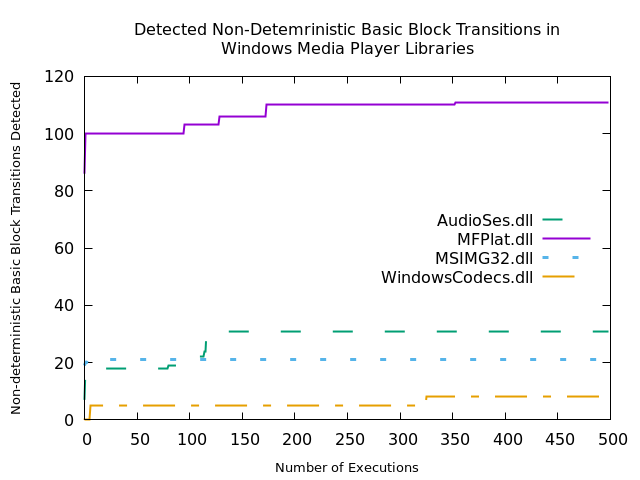
\includegraphics[width=3.5in]{picker.png}
\caption{Total Non-deterministic Basic Block Transitions Detected per Execution In Windows Media Player Libraries}
\label{fig:picker}
\end{figure}

The algorithm the Picker uses is not effective with all instrumentation
modules. The Picker uses the instrumentation module which will be used in
practice, and uses the same options for that module. It then operates on
the opaque blob which represents the code coverage information.  It does
this without any knowledge of the internal format.  Anything which uses the
\AFL{}-style bitmap will work fine.  This would include the DynamoRIO and
\AFL{} instrumentation modules. The \IPT{} instrumentation output is the hashes
of the \TNT{} and \TIP{} packets, so any non-determinism will change every byte of
the instrumentation data.  This will cause the Picker to mask out all bytes of
the coverage data, which is not useful. If the Intel PT
instrumentation was also a tracer, it would be capable of using an internal
format which is compatible with the Picker.
